\subsection{Android overview}

Android applications are typically programmed from Integrated Development Environments (IDE) such as  Eclipse or Android Studio. The latter has been used in this because it is the official Android IDE supported by Google \cite{component16}.\\

The typical app skeleton is shown in Figure \ref{androidActivity} \cite{component17}. It consists of the following functions:

	\begin{itemize}

	\item \textbf{onCreate()} \hfill \\
	The first function Android calls when the application is launched. Here is where all the static elements are defined, such as setting the views.
	
	\item \textbf{onStart()} \hfill \\
	This function is called when the app is first visible to the user, after the previous function has ended.


	\item \textbf{onResume()} \hfill \\
	This method is called when the app is ready to interact with the user, ie. it is on top of the application stack and receives the user input.

	\item \textbf{onPause()} \hfill \\
	This is called when a previously started activity is going to be resumed. It is typically used to save data and stop resource consuming parts such as animations.

	\item \textbf{onStop()} \hfill \\
	Called when the activity is no longer visible to the user, either because another activity or the current one is being destroyed.

	\item \textbf{onRestart()} \hfill \\
	It is called when the activity is has been stopped, before it is restarted.

	\item \textbf{onDestroy()} \hfill \\
	If the activity is not restarted it is destroyed. It is the final function used in the activity and is called either explicitly with the \textit{finish()} method or because the system closes it because it is low on resources.


	\end{itemize}
	\bigskip
	
	
	\begin{figure}[H]
      \centering
      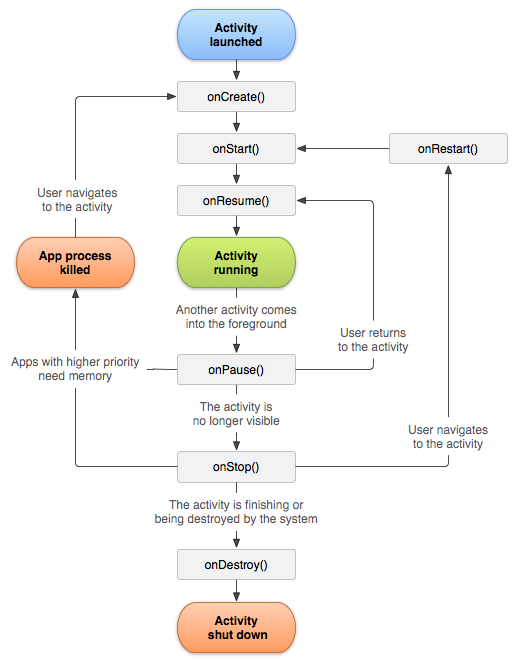
\includegraphics[scale=.8]{images/Diagrams/android_activity_lifecycle.png}
      \caption{Android app activity lifecycle }
      \label{androidActivity}
  	\end{figure}
  	\bigskip



% \begin{figure}[H]
%       \centering
%       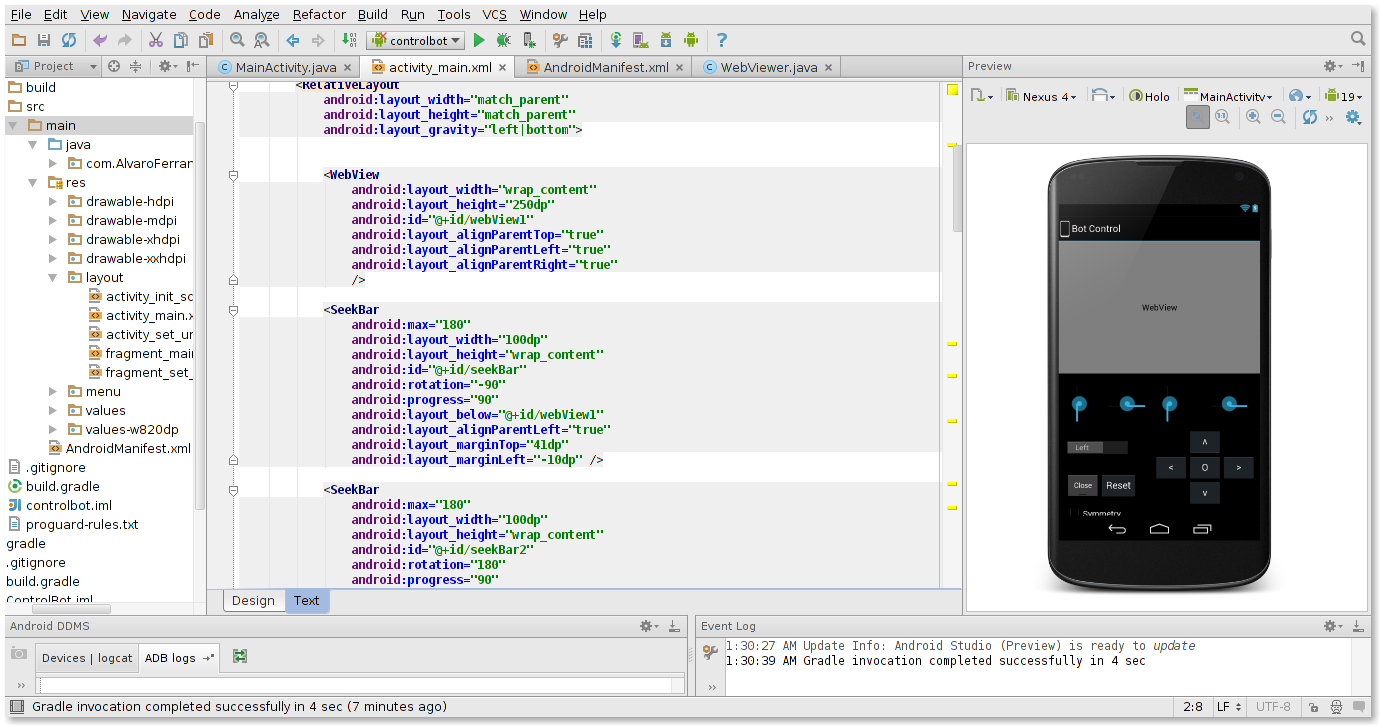
\includegraphics[scale=.3]{images/Android/androidStudio.png}
%       \caption{Android Studio IDE }
%       \label{androidStudio}
%   \end{figure}
%   \bigskip

\newpage
\subsection{Bot Control}

The robot is controlled from the Android application Bot Control, seen in Figure \ref{BotControlApp}. As it can be seen it is divided in two halves, with the upper half displaying the video received from the bot and the lower one encompassing the controls. The complete list of widgets include:

	\begin{itemize}
	\item A WebView connected to the url given by MJPG-Streamer which displays the video feed streamed from the webcam

	\item Four SeekBars, used to select the desired angle for each of the servomotors that position the arms

	\item A "Left/Right" Switch for selecting between the left and right arms

	\item A "Close" Button to close the claw of the current arm

	\item A "Reset" Button to reset the position of the arms, turning each servo at 90 degrees

	\item A "Symmetry" CheckBox to activate said option, under which both arms are controlled simultaneously and symetrically

	\item Five direction Buttons to navigate the robot, which result in it moving forwards or backwards, turning left or right and stopping in place

	\end{itemize}
 

	\begin{figure}[H]
      \centering
      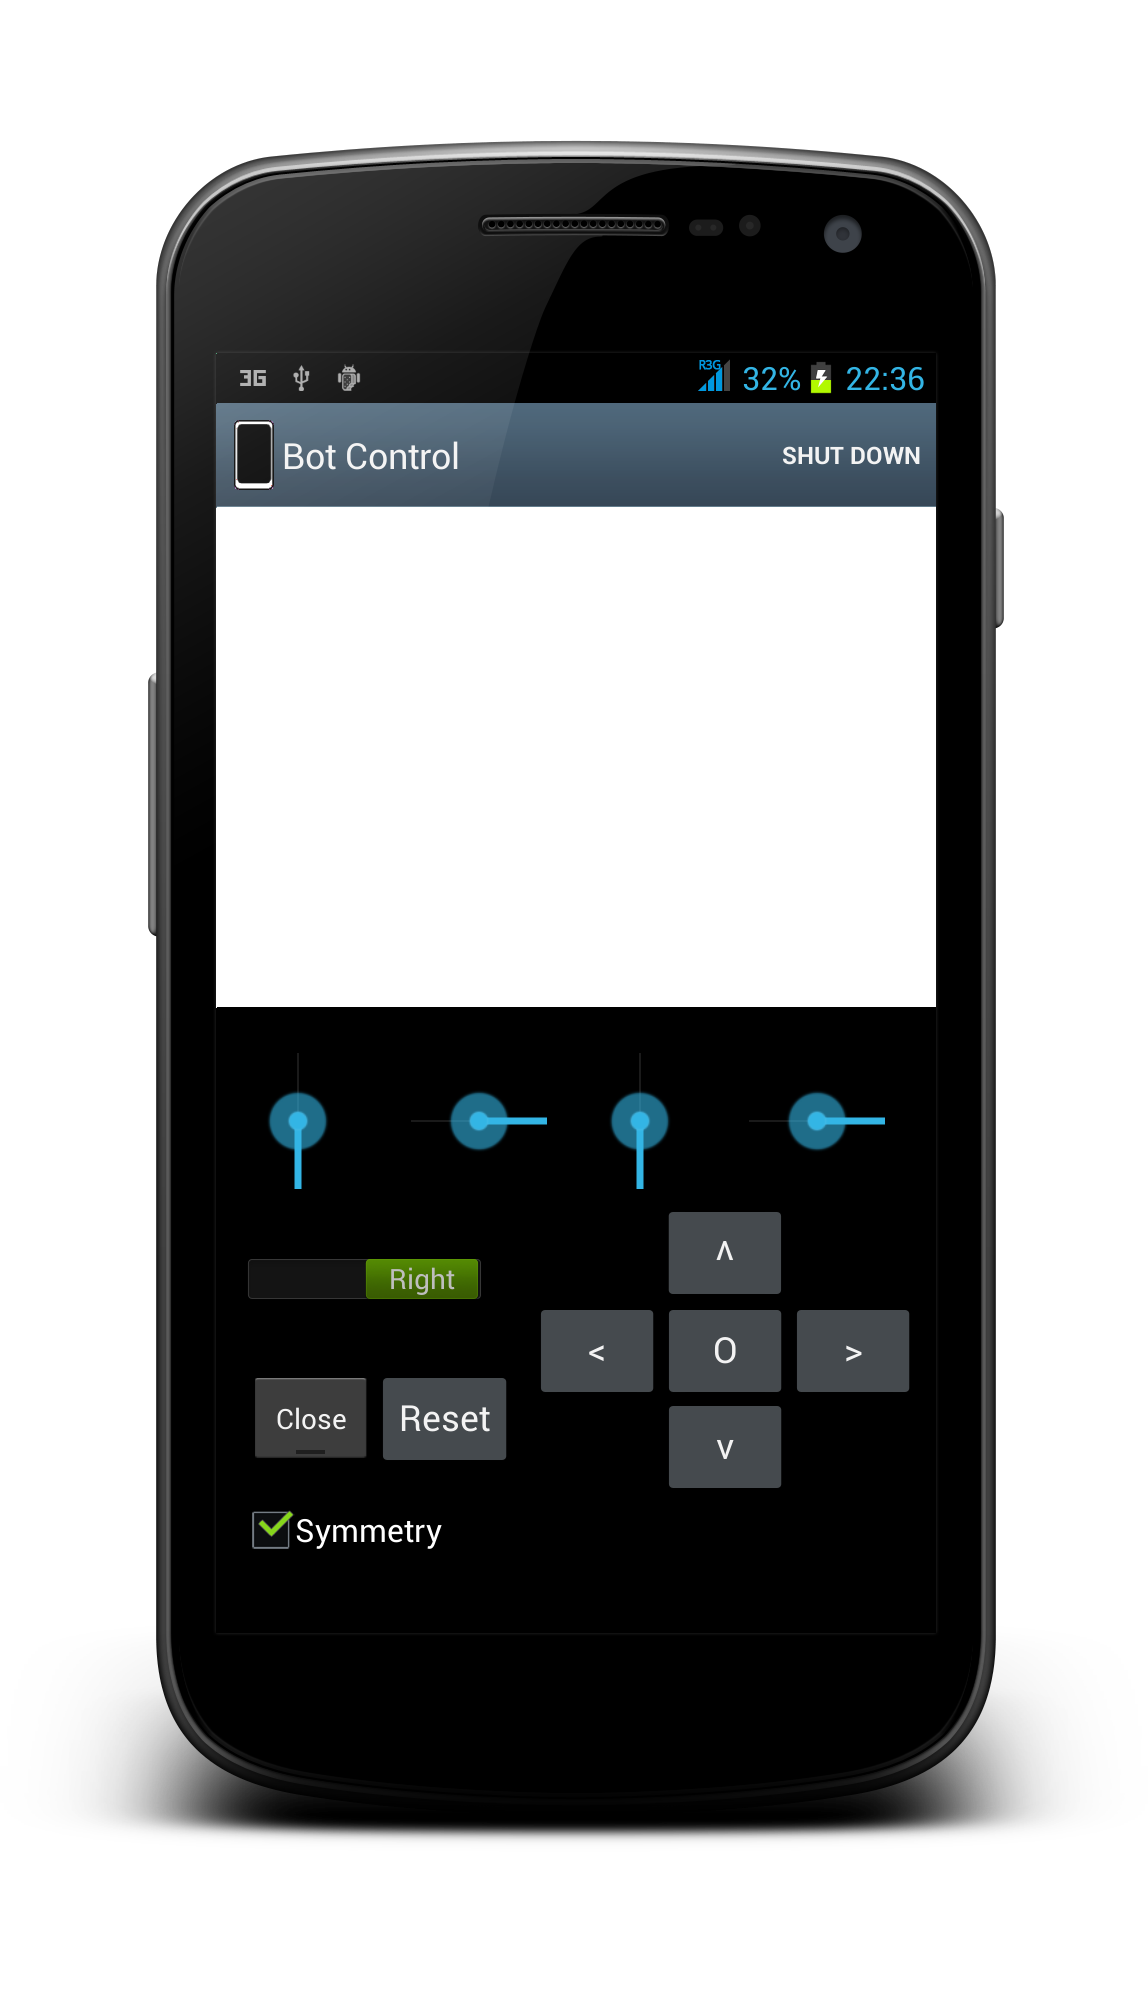
\includegraphics[scale=.17]{images/Android/BotControl.png}
      \caption{Bot Control application }
      \label{BotControlApp}
  \end{figure}
  \bigskip


The application follows the same general structure presented in the previous section. Here each function used will be analyzed if their default behaviour has been overridden. The following is a list of the modified functions specified in the program's code.
 
	\begin{itemize}

	\item \textbf{onCreate()} \hfill \\
	This is the first function called upon start. The clientThread class is started here and the WebView connects to the robot's IP to reproduce the video stream.
	\\

	% \item \textbf{onResume()} \hfill \\
	% This is ...


	\end{itemize}

\bigskip

The "Activity running" state is in this case composed by two separate functions, as illustrated by Figure \ref{activityDetail}.

	\begin{figure}[H]
      \centering
      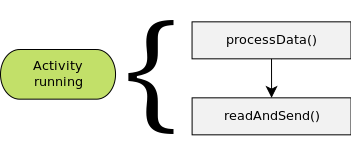
\includegraphics[scale=.8]{images/Diagrams/androidActivity.png}
      \caption{Detail of the "Activity running" state}
      \label{activityDetail}
	\end{figure}

\bigskip

	\begin{itemize}

	\item \textbf{processData()} \hfill \\
	This function identifies and stores changes in movement parameters, such as those resulting in arm or body movement, and calls \textit{readAndSend()} to send them to the robot.\\

	\item \textbf{readAndSend()} \hfill \\
	This function is in charge of reading the values of non-movement parameters, such as symmetry or side selection, and sends these and the previous to the robot through the socket.\\

	\item \textbf{onStop()} \hfill \\
	This is the last function to be called before the activity's destruction. It closes the socket after sending the "quit" keyword that tells the Raspberry Pi to start looking for clients again. \\

	\item \textbf{clientThread} \hfill \\
	The runnable class \textit{clientThread} is in charge of creating a socket client that will be used to send commands over wifi.\\

	\end{itemize}

\bigskip

In conclusion, Bot Control sends information on the movements the robot needs to deliver while it displays what the latter sees, in order to be able to perform actions like grabbing a bottle from one room and navigating back to the user without having to follow it around the house.